\documentclass{article}
\usepackage{fancyhdr}
\usepackage{ctex}
\usepackage{listings}
\usepackage{graphicx}
\usepackage[a4paper, body={18cm,22cm}]{geometry}
\usepackage{amsmath,amssymb,amstext,wasysym,enumerate,graphicx}
\usepackage{float,abstract,booktabs,indentfirst,amsmath}
\usepackage{array}
\usepackage{booktabs}
\usepackage{multirow}
\usepackage{url}
\usepackage{diagbox}
\renewcommand\arraystretch{1.4}
\usepackage{indentfirst}
\setlength{\parindent}{2em}
\usepackage{enumitem}
\setmonofont{DejaVu Sans Mono}
\usepackage{listings}
\usepackage{xcolor}
\usepackage{makecell}
\setCJKmonofont{黑体}
\usepackage{tikz}
\usepackage{tabularx}
\usepackage{amsmath}
\usetikzlibrary{positioning, arrows.meta}
\lstset{
    % language = C,
    xleftmargin = 3em,xrightmargin = 3em, aboveskip = 1em,
	backgroundcolor = \color{white}, % 背景色
	basicstyle = \small\ttfamily, % 基本样式 + 小号字体
	rulesepcolor= \color{gray}, % 代码块边框颜色
	breaklines = true, % 代码过长则换行
	numbers = left, % 行号在左侧显示
	numberstyle = \small, % 行号字体
    numbersep = -14pt, 
    keywordstyle=\color{purple}\bfseries, % 关键字颜色
    commentstyle =\color{red!50!green!50!blue!60}, % 注释颜色
    stringstyle = \color{red}, % 字符串颜色
    morekeywords={ASSERT, int64_t, uint32_t},
	frame = shadowbox, % 用(带影子效果)方框框住代码块
	showspaces = false, % 不显示空格
	columns = fixed, % 字间距固定
} 
\lstset{
    sensitive=true,
    moreemph={ASSERT, NULL}, emphstyle=\color{red}\bfseries,
    moreemph=[2]{int64_t, uint32_t, tid_t, uint8_t, int16_t, uint16_t, int32_t, size_t}, emphstyle=[2]\color{purple}\bfseries,
    }
%--------------------页眉--------------------%
\pagestyle{fancy}
\fancyhead[L]{华东师范大学}
\fancyhead[R]{East China Normal University}
\fancyhead[C]{}
\fancyfoot[C]{-\thepage-}
\renewcommand{\headrulewidth}{1.5pt}
%--------------------标题--------------------%
\begin{document}
\begin{center}
  \LARGE{{\textbf{\heiti 华东师范大学软件工程学院实验报告}}}
  \begin{table}[H]
    \centering
    \begin{tabular}{p{2cm}p{4cm}<{\centering}p{1cm}p{2cm}p{4cm}<{\centering}}
      实验课程:    & 计算机网络 & \quad & 年\qquad 级: & 2023级      \\ \cline{2-2} \cline{5-5}
      实验编号:    & Lab 06     & \quad & 实验名称:    & TCP
      \\ \cline{2-2} \cline{5-5}
      姓\qquad 名: & 王海生     & \quad & 学\qquad 号: & 10235101559 \\ \cline{2-2} \cline{5-5}
    \end{tabular}
  \end{table}
\end{center}
\rule{\textwidth}{1pt}

\tableofcontents

%--------------------正文--------------------%
\section{实验目的}
\begin{enumerate}[noitemsep, label={{\arabic*})}]
  \item 学会通过 \texttt{Wireshark}获取 \texttt{TCP}消息
  \item 掌握 \texttt{TCP}数据包结构
  \item 掌握 \texttt{TCP}数据包各字段的含义
  \item 掌握 \texttt{TCP}连接建立和释放的步骤
  \item 掌握 \texttt{TCP}数据传输阶段的过程
\end{enumerate}
\section{实验内容与实验步骤}
\subsection{实验内容}

\subsubsection{捕获 \texttt{TCP} 报文}

\begin{enumerate}[noitemsep]
  \item 以 \url{http://old.ecnu.edu.cn/site/xiaoli/2016.jpg}为例,用 \texttt{wget}确认该链接有效。
  \item 启动\texttt{Wireshark},在菜单栏的捕获 \( \to \) 选项中进行设置,选择已连接的以太网,设置捕获过滤器为\texttt{tcp and host old.ecnu.edu.cn}。我们主要观察客户端与服务器之间的\texttt{tcp}流。
  \item 捕获开始后,重复第一步,重新发送请求。
  \item 当\texttt{wget}命令结束后,停止\texttt{Wireshark}捕获。
\end{enumerate}

\subsubsection{分析 \texttt{TCP} 报文}

选择一个TCP帧,观察其协议层:

\begin{enumerate}[noitemsep]
  \item 根据你的理解,绘制\texttt{TCP}报文段的结构图(包括头部各字段的位置及大小)。
\end{enumerate}

\subsubsection{\texttt{TCP} 连接的建立和释放}

TCP的三次握手协议主要分为以下三个步骤:
\begin{enumerate}[noitemsep]
  \item 客户端发送一个\texttt{SYN}包给服务器,然后等待应答。
  \item 服务器端回应给客户端一个\texttt{ACK=1}、\texttt{SYN=1}的\texttt{TCP}数据段。
  \item 客户必须再次回应服务器端一个\texttt{ACK}确认数据段。
\end{enumerate}

在你捕获到的结果中,找到设置了\texttt{SYN}标志的\texttt{TCP}段及其后的数据包,完成以下问题: 

\begin{enumerate}[noitemsep]
  \item 绘制三次握手的时序图,直到并包括建立连接后计算机发送的第一个数据包(\texttt{HTTP GET}请求),包括:
  \begin{itemize}
  	\item 每个数据段的序列号和\texttt{Ack}标号;
  	\item 本地计算机发送或接收每个数据段的时间(以毫秒为单位);
  	\item 本地计算机从发送\texttt{SYN}段到接收到\texttt{SYN-ACK}段的往返时间。
  \end{itemize}
  \item \texttt{SYN}数据包上携带哪些\texttt{TCP}选项?
\end{enumerate}

\texttt{TCP}的四次挥手主要分为以下四个步骤:
\begin{enumerate}[noitemsep]
  \item 客户端进程发出断开连接指令,这将导致客户端的\texttt{TCP}程序创建一个特殊的\texttt{TCP}报文段,发送到服务器。这个报文段的\texttt{FIN}字段被置为1,表示这是一条断开连接的报文;
  \item 服务器接收到客户端发来的断开连接报文,向客户端回送这个报文的确认报文(\texttt{ACK}字段为1),告诉服务器已经接收到\texttt{FIN}报文,并允许断开连接;
  \item 服务器发送完确认报文后,服务器的\texttt{TCP}程序创建一条自己的断开连接报文,此报文的\texttt{FIN}字段被置为1,然后发往客户端;
  \item 客户端接收到服务器发来的\texttt{FIN}报文段,则产生一条确认报文(\texttt{ACK}为1),发送给服务器,告知服务器已经接收到了它的断开报文。服务器接收到这条\texttt{ACK}报文段后,释放\texttt{TCP}连接相关的资源(缓存和变量),而客户端等待一段时间后(半分钟、一分钟或两分钟),也释放处于客户端的缓存和变量。
\end{enumerate}

回答问题:
\begin{enumerate}[noitemsep]
  \item 传输完成后,\texttt{TCP}连接会以四次挥手或一端发送\texttt{RST}数据包的方式断开,同1一样,绘制\texttt{TCP}连接释放的时序图(从发出第一个\texttt{FIN}或\texttt{RST}到连接断开为止)。
\end{enumerate}

\subsubsection{TCP 数据传输}

在“统计”菜单下,选择“ IO图表”,以查看数据包速率。

\begin{itemize}
	\item 调整过滤器为“\texttt{tcp.srcport==80}”仅查看下载数据包,重新绘图;
	\item 调整过滤器为“\texttt{tcp.dstport==80}”仅查看上传数据包,重新绘图;
\end{itemize}

通过你对数据传输的理解,回答以下问题:

\begin{enumerate}[label={\arabic*)}, noitemsep]
  \item 实验中下载的大概速率为多少?(以\texttt{packets/s}和\texttt{bits/s}为单位)
  \item 下载内容(即\texttt{TCP}有效负载)占下载率的百分比是多少?
  \item 实验中上传的大概速率为多少?(以\texttt{packets/s}和\texttt{bits/s}为单位)
  \item 如果最近从服务器收到的 \texttt{TCP} 数据段的序列号是 $X$,那么下一个发送的 \texttt{ACK} 是多少?
\end{enumerate}

\subsubsection{问题讨论}

\begin{enumerate}[noitemsep]
  \item 探索\texttt{TCP}的拥塞控制和经典\texttt{AIMD}策略。
  \item 更深入地探索\texttt{TCP}的可靠性机制。捕获包括段丢失的\texttt{TCP}连接,查看什么触发重新传输以及何时触发,另外查看往返时间估算工具。
  \item 查看包括\texttt{SACK}在内的选项的使用以了解详细信息。
  \item \texttt{TCP}是\texttt{Web}的基础传输层。可以通过设置并发连接来查看浏览器如何使用\texttt{TCP}。
\end{enumerate}


\subsection{实验步骤}

\begin{enumerate}[noitemsep]
  \item 以 \url{http://old.ecnu.edu.cn/site/xiaoli/2016.jpg}为例,用 \texttt{wget}确认该链接有效
  \begin{lstlisting}
    PS> wget http://old.ecnu.edu.cn/site/xiaoli/2016.jpg
  \end{lstlisting}
  \item 启动\texttt{Wireshark},在菜单栏的捕获 \( \to \) 选项中进行设置,选择已连接的以太网,设置捕获过滤器为\texttt{tcp and host img.zcool.cn}。我们主要观察客户端与服务器之间的\texttt{tcp}流。
  \item 捕获开始后,重复第一步,重新发送请求。
  \item 当\texttt{wget}命令结束后,停止\texttt{Wireshark}捕获。
  \item 分析 \texttt{TCP} 报文
\end{enumerate}

\section{实验环境}


\begin{itemize}[noitemsep]
  \item 操作系统:\texttt{Windows 11 家庭中文版 23H2 22631.2715}
  \item 网络适配器:\texttt{Killer(R) Wi-Fi 6 AX1650i 160MHz Wireless Network Adapter(201NGW)}
  \item \texttt{Wireshark}:\texttt{Version 4.2.0 (v4.2.0-0-g54eedfc63953)}
  \item \texttt{wget}:\texttt{GNU Wget 1.21.4 built on mingw32}
\end{itemize}


\section{实验结果与分析}

\subsection{捕获 \texttt{TCP} 报文}

首先,我们使用 \texttt{wget} 命令,发现链接已经失效。

\begin{figure}[H]
  \centering
  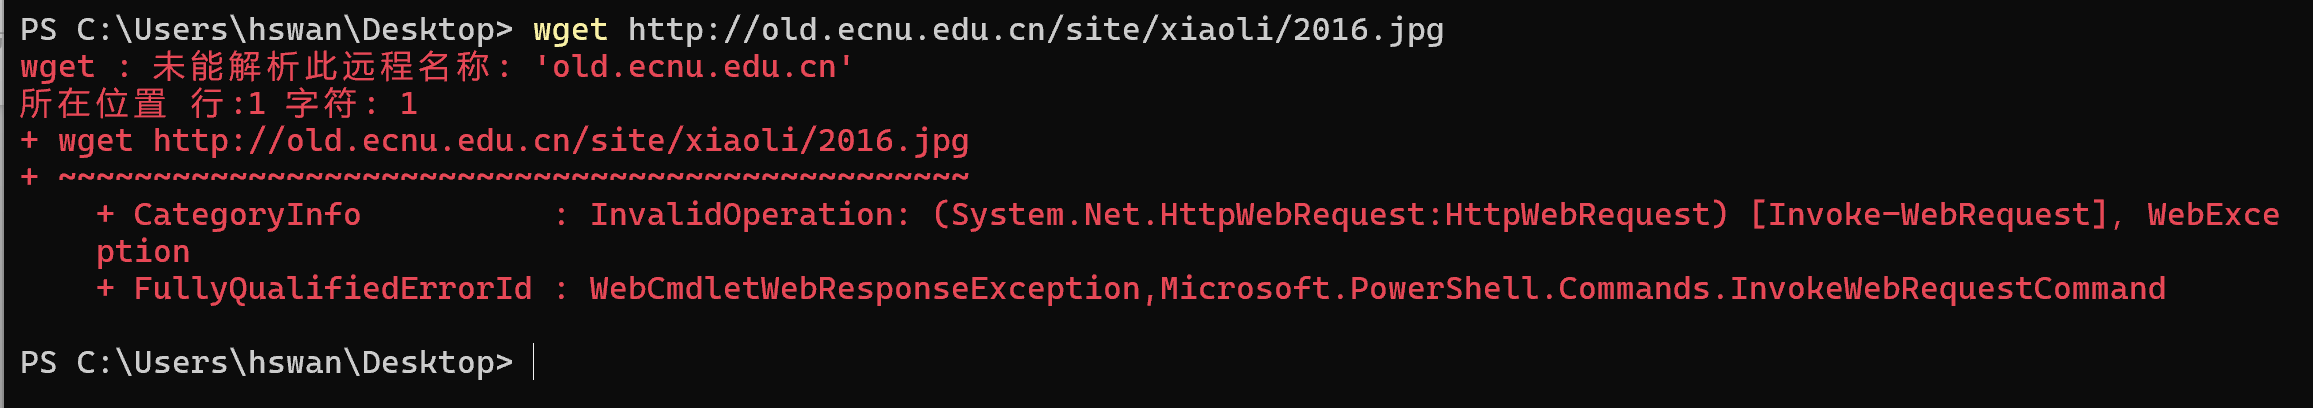
\includegraphics[width=0.9\textwidth]{img/1.png}
  \caption{链接失效}
\end{figure}

接着尝试\url{http://img.zcool.cn/community/01dcd059117b12a801216a3e9c4fd5.jpg},发现链接有效。

\begin{lstlisting}
	wget http://img.zcool.cn/community/01dcd059117b12a801216a3e9c4fd5.jpg
	--2024-12-16 09:04:31--  http://img.zcool.cn/community/01dcd059117b12a801216a3e9c4fd5.jpg
	Resolving img.zcool.cn (img.zcool.cn)... 116.211.153.215, 150.139.142.248, 182.40.32.241, ...
	Connecting to img.zcool.cn (img.zcool.cn)|116.211.153.215|:80 ... connected.
	HTTP request sent, awaiting response... 301 Moved Permanently
	Location: https://img.zcool.cn/community/01dcd059117b12a801216a3e9c4fd5.jpg [following]
	--2024-12-16 09:04:31--  https://img.zcool.cn/community/01dcd059117b12a801216a3e9c4fd5.jpg
	Connecting to img.zcool.cn (img.zcool.cn)|116.211.153.215|:443 ... connected.
	HTTP request sent, awaiting response... 200 OK
	Length: 1647322 (1.6M) [image/jpeg]
	Saving to: '01dcd059117b12a801216a3e9c4fd5.jpg.1'
	
	01dcd059117b12a801216a3e9c4fd5 100%[======================================>] 1.57M --.-KB/s    in 0.1s
	
	2024-12-16 09:04:31 (11.9 MB/s) - '01dcd059117b12a801216a3e9c4fd5.jpg.1' saved [1647322/1647322]
\end{lstlisting}

然后,我们启动\texttt{Wireshark},在菜单栏的捕获 \( \to \) 选项中进行设置,选择已连接的以太网,设置捕获过滤器为\texttt{tcp and host img.zcool.cn}。我们主要观察客户端与服务器之间的\texttt{tcp}流。

\begin{figure}[H]
  \centering
  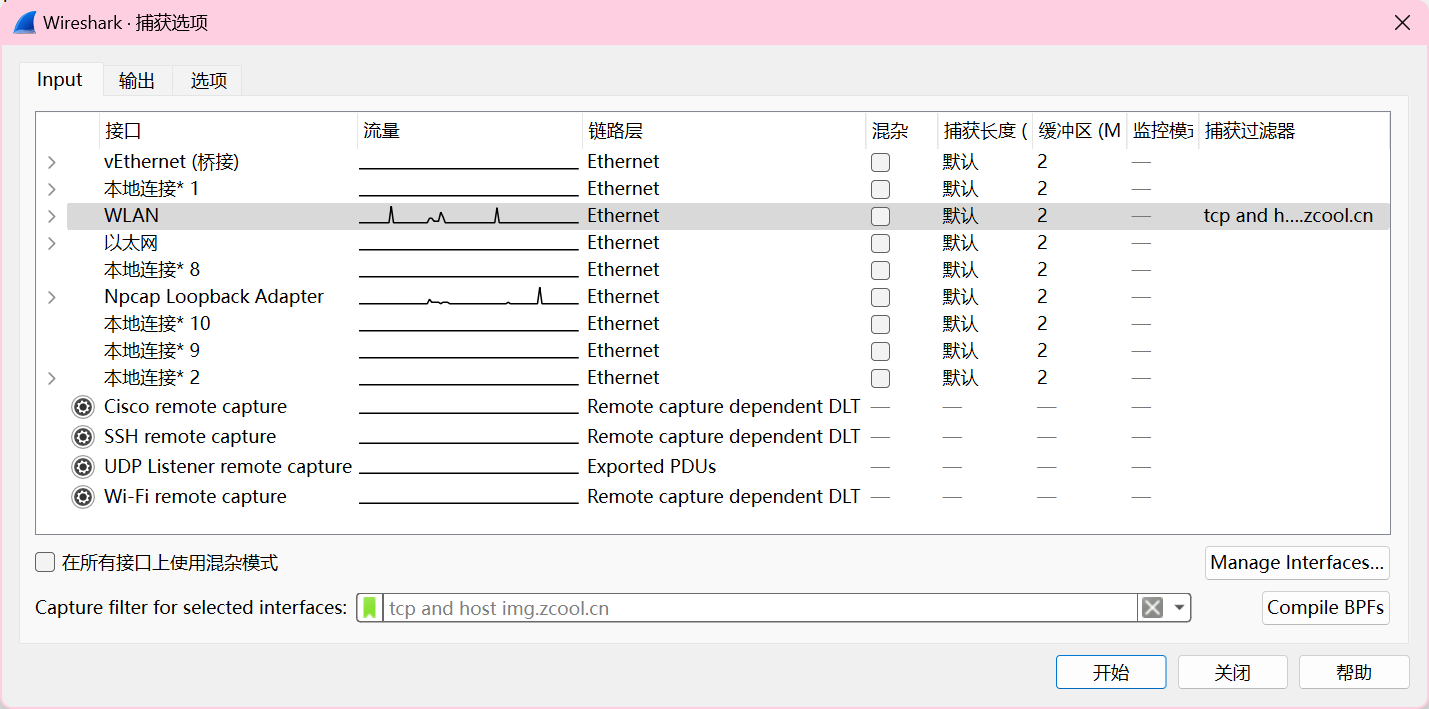
\includegraphics[width=0.8\textwidth]{img/2.png}
  \caption{设置捕获过滤器}
\end{figure}

捕获开始后,重复第一步,重新发送\texttt{wget}请求。

当\texttt{wget}命令结束后,停止\texttt{Wireshark}捕获。
捕获结果如下:

\begin{figure}[H]
  \centering
  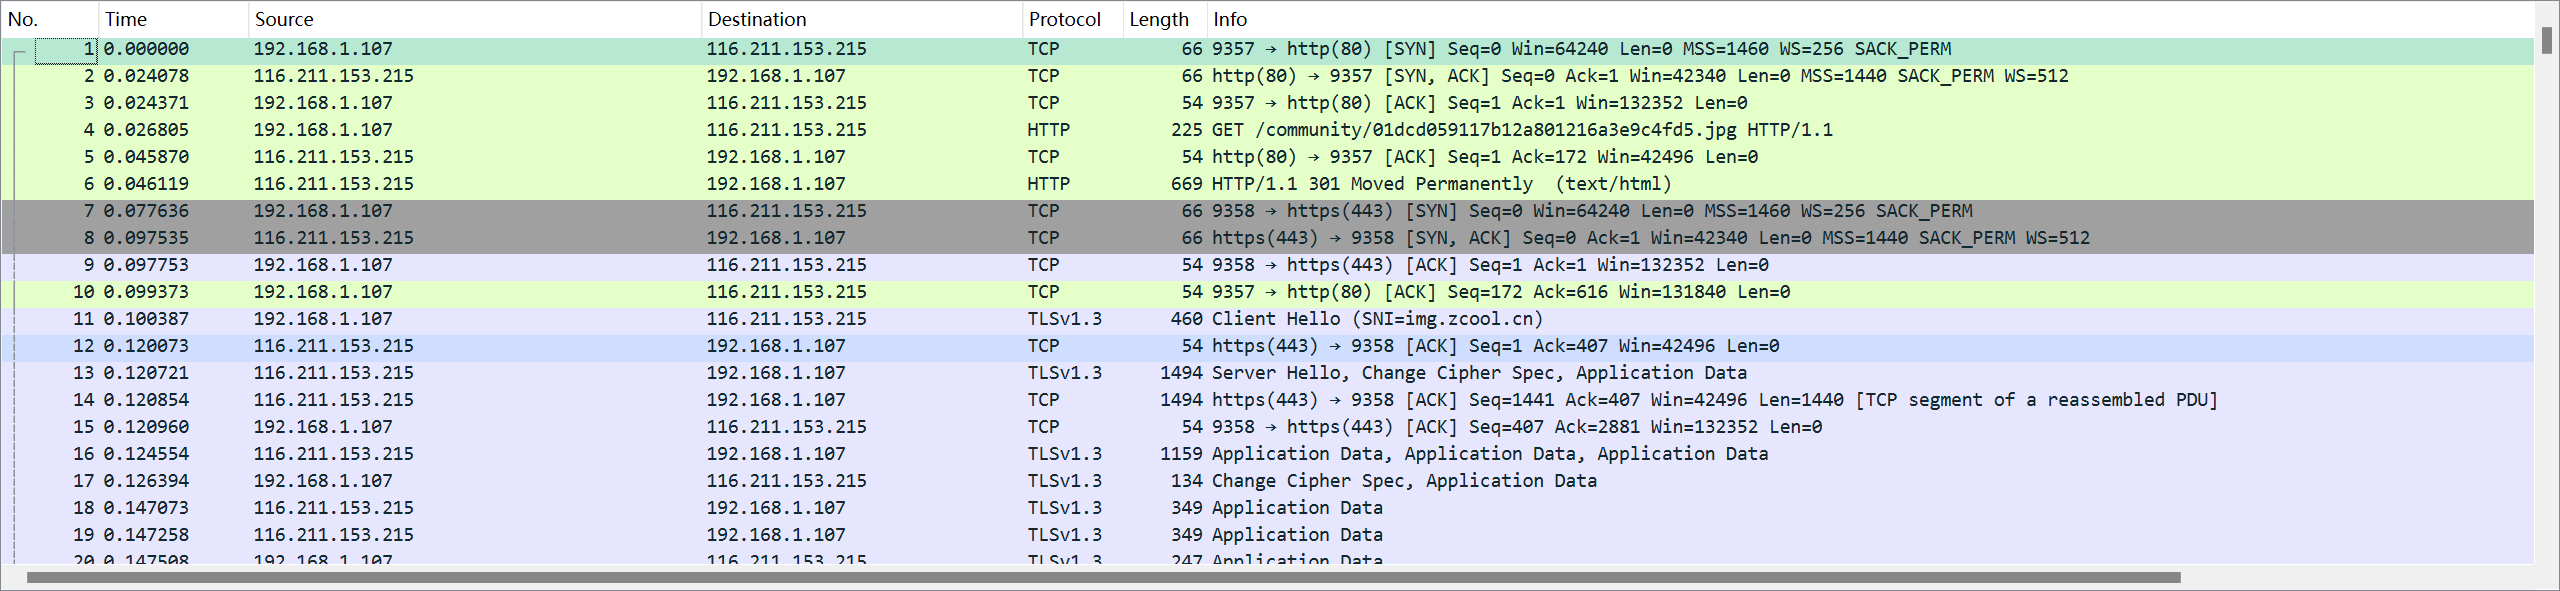
\includegraphics[width=0.8\textwidth]{img/4.png}
  \caption{捕获结果}
\end{figure}


\subsection{\texttt{TCP}报文段的结构}

选择一个\texttt{TCP}数据包,如下所示:

\begin{figure}[H]
  \centering
  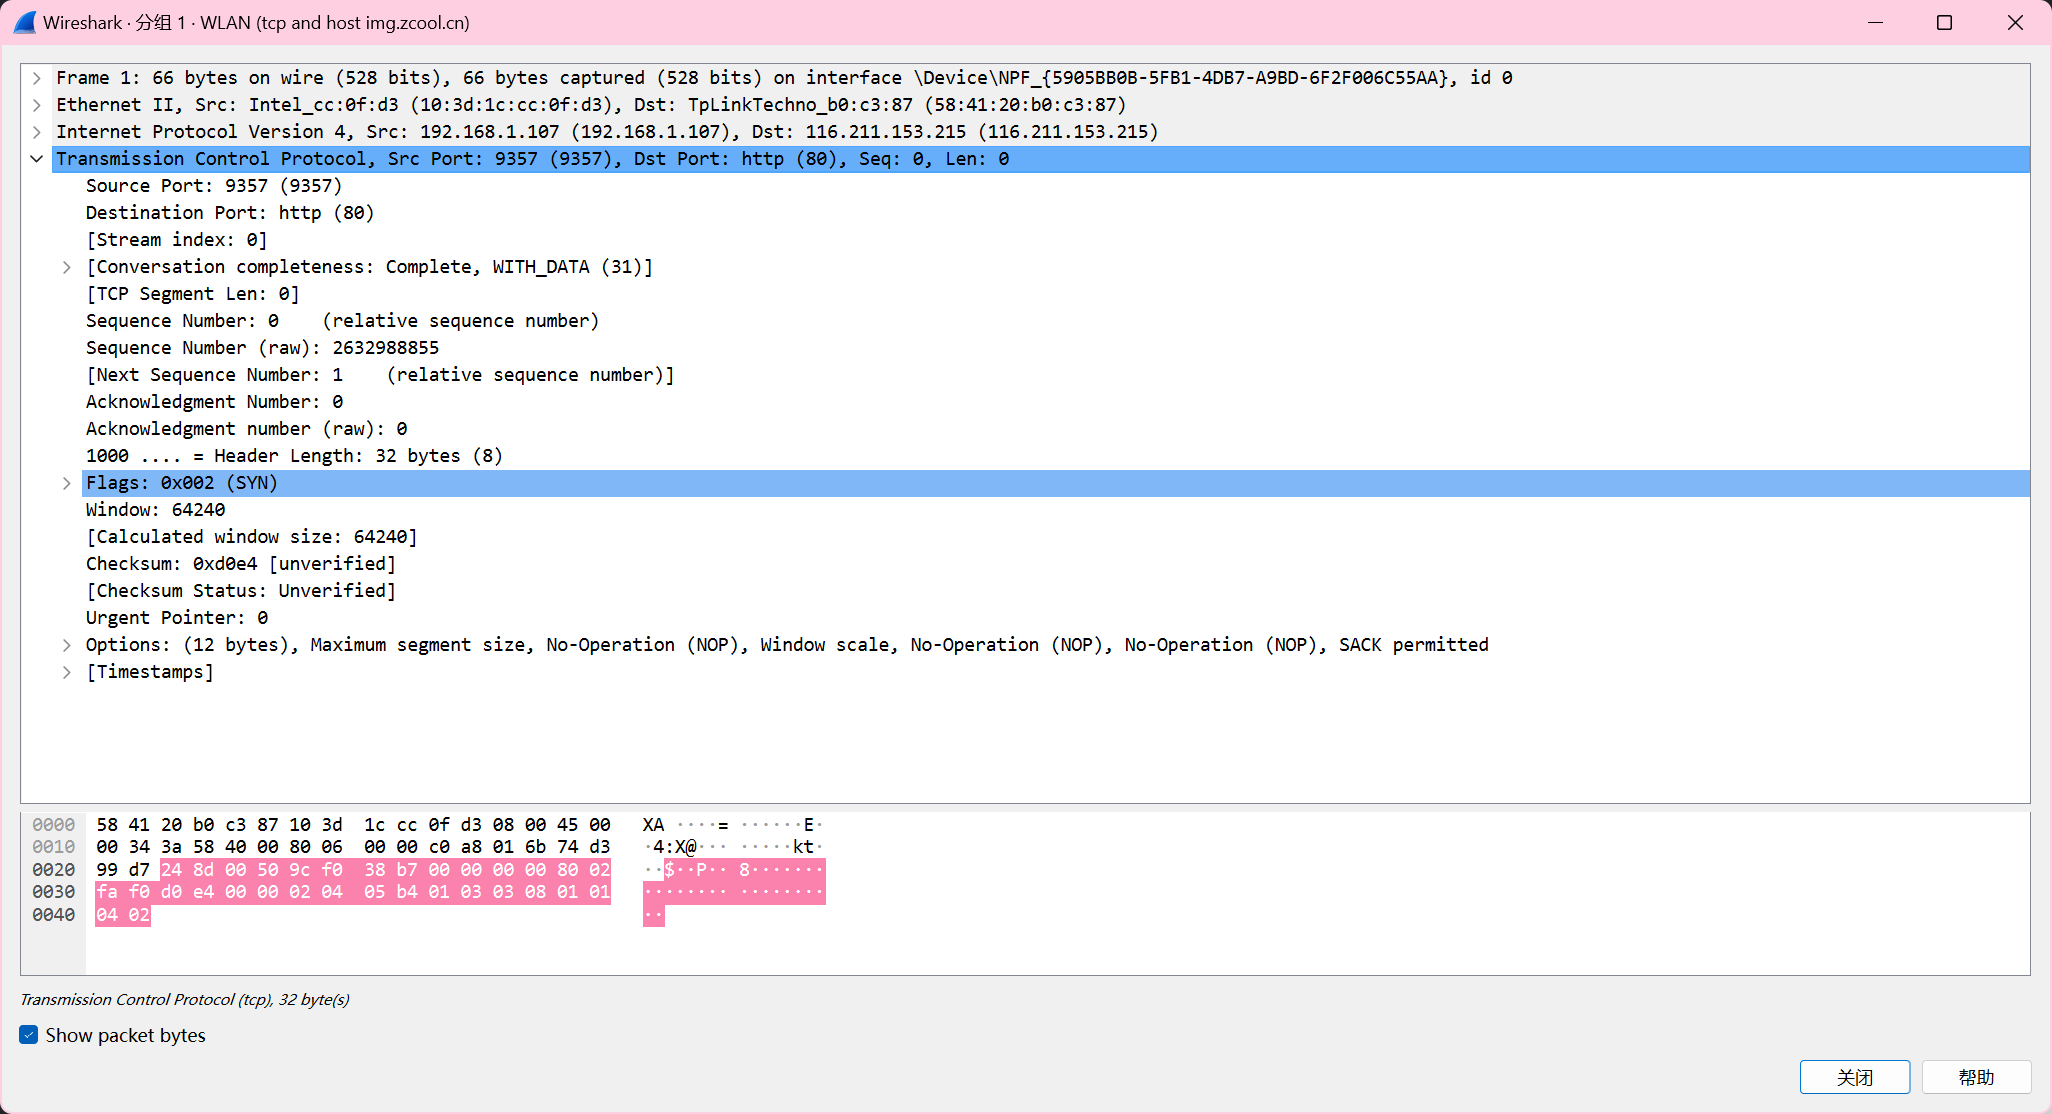
\includegraphics[width=0.79\textwidth]{img/5.png}
  \caption{一个\texttt{TCP}数据包}
\end{figure}

可以画出\texttt{TCP}包的结构如下:

% 八列的表格
\begin{table}[H]
  \centering
  \begin{tabularx}{0.8\textwidth}{|*{4}{X|}}
    \hline
    \multicolumn{2}{|X|}{源端口 Source Port}     & \multicolumn{2}{X|}{目的端口 Destination Port}                                          \\
    \multicolumn{2}{|X|}{2 bytes}                & \multicolumn{2}{X|}{2 bytes}                                                            \\
    \hline
    \multicolumn{4}{|X|}{序列号 Sequence Number}                                                                                           \\
    \multicolumn{4}{|X|}{4 bytes}                                                                                                          \\
    \hline
    \multicolumn{4}{|X|}{确认号 Acknowledgment Number}                                                                                     \\
    \multicolumn{4}{|X|}{4 bytes}                                                                                                          \\
    \hline
    \multicolumn{1}{|X|}{头部长度 Header Length} & \multicolumn{1}{X|}{标志 Flags}                & \multicolumn{2}{X|}{窗口大小 Window}   \\
    \multicolumn{2}{|X|}{共 2 bytes}             & \multicolumn{2}{X|}{2 bytes}                                                            \\
    \hline
    \multicolumn{2}{|X|}{校验和 Checksum}        & \multicolumn{2}{X|}{紧急指针 Urgent Pointer}                                            \\
    \multicolumn{2}{|X|}{2 bytes}                & \multicolumn{2}{X|}{2 bytes}                                                            \\
    \hline
    \multicolumn{4}{|X|}{可选项 Options}                                                                                                   \\
    \multicolumn{4}{|X|}{0-40 bytes}                                                                                                       \\
    \hline
                                                 &                                                &                                      & \\
    \hline
    \multicolumn{4}{|X|}{负载 Payload}                                                                                                     \\
    \multicolumn{4}{|X|}{n bytes}                                                                                                          \\
    \hline
  \end{tabularx}
  \caption{\texttt{TCP}报文段的结构图}
\end{table}

其中 \texttt{Flags} 字段包括 \texttt{Reserved}, \texttt{Accurate ECN}, \texttt{Congestion Window Reduced}, \texttt{ECN-Echo}, \\ \texttt{Urgent}, \texttt{Acknowledgment}, \texttt{Push}, \texttt{Reset}, \texttt{Syn}, \texttt{Fin}。


\texttt{TCP}数据包头部各字段的含义如下:

\begin{itemize}[noitemsep]
  \item 源端口:源端口号,占2字节,用来标识源主机的应用程序进程。
  \item 目的端口:目的端口号,占2字节,用来标识目的主机的应用程序进程。
  \item 序列号:占4字节,用来标识从TCP源端向目的端发送的字节流,发起方发送数据时对此进行标记。
  \item 确认号:占4字节,只有ACK标志位为1时,确认号字段才有效,确认号等于上次接收到的字节序号加1。
  \item 头部长度:占1字节,指示TCP头部长度。
  \item 标志:与头部长度合占2字节。各标志位的含义如下:
        \begin{itemize}[noitemsep]
          \item Reserved:保留位。
          \item Accurate ECN:显式拥塞通知。
          \item Congestion Window Reduced:拥塞窗口减小。
          \item ECN-Echo:显式拥塞通知回显。
          \item URG:紧急指针(urgent pointer)有效。
          \item ACK:确认序号有效。
          \item PSH:接收方应该尽快将这个报文交给应用层。
          \item RST:重置连接。
          \item SYN:发起一个新连接。
          \item FIN:释放一个连接。
        \end{itemize}
  \item 窗口大小:占2字节,窗口大小是指发送方在收到确认前允许发送的字节数。
  \item 校验和:占2字节,检验TCP首部和TCP数据的正确性。
  \item 紧急指针:占2字节,仅当URG标志为1时,紧急指针才有效。紧急指针告诉系统此报文段中有紧急数据,紧急数据的字节数由紧急指针指出。
  \item 可选项:占0-40字节,可选项可以有0个或多个,用于一些可选的设置。
\end{itemize}

\subsection{\texttt{TCP} 连接的建立和释放}

\subsubsection{三次握手的时序图}

我们知道,三次握手的过程如下:

\begin{enumerate}[noitemsep]
  \item 客户端发送一个\texttt{SYN}包给服务器,然后等待应答。
  \item 服务器端回应给客户端一个\texttt{ACK=1}、\texttt{SYN=1}的\texttt{TCP}数据段。
  \item 客户必须再次回应服务器端一个\texttt{ACK}确认数据段。
\end{enumerate}

在 \texttt{Wireshark} 中,我们可以看到三次握手的过程如下:

\begin{figure}[H]
  \centering
  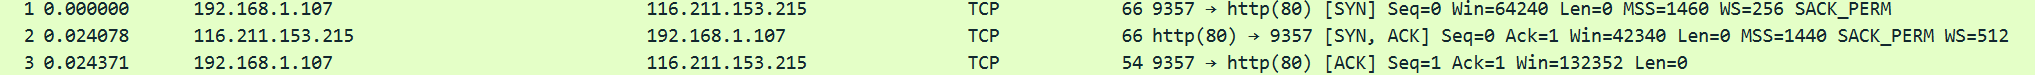
\includegraphics[width=0.95\textwidth]{img/6.png}
  \caption{三次握手}
\end{figure}

画出三次握手协议的步骤图如下:

\begin{figure}[H]
  \centering
  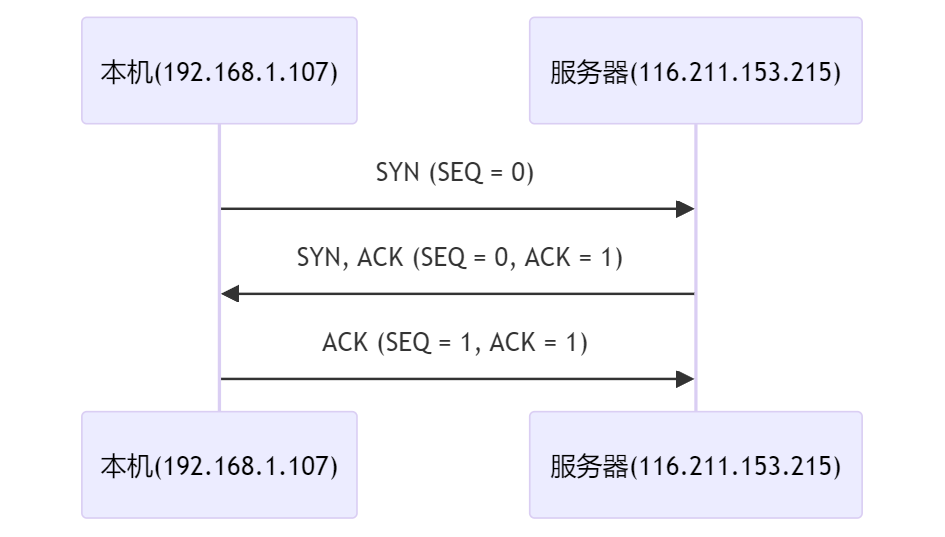
\includegraphics[width=0.95\textwidth]{img/7.png}
  \caption{三次握手协议的步骤图}
\end{figure}

\subsubsection{\texttt{SYN}数据包上携带的\texttt{TCP}选项}

在\texttt{TCP}连接建立过程中,\texttt{SYN}数据包用于初始化连接,并携带多种\texttt{TCP}选项:

\begin{enumerate}
	\item \texttt{Maximum Segment Size (MSS)}
	
	定义了在这个连接上发送的\texttt{TCP}段中最大的数据量(不包括\texttt{TCP}头部)。接收端通过这个选项告诉发送端它能接受的最大段大小,从而避免分片。
	
	\item \texttt{Window Scale Option}
	
	允许窗口大小超过65,535字节。它通过指定一个移位计数来扩大窗口尺寸,这使得\texttt{TCP}能够在高速、高延迟的网络上有效地工作。
	
	\item \texttt{SACK Permitted}
	
	\texttt{Selective Acknowledgment}允许接收方通知发送方哪些数据已经成功接收,哪些数据丢失需要重传。这样可以提高效率,因为不需要重传所有未确认的数据。
	
	\item \texttt{Timestamps}
	
	时间戳选项提供了一种测量往返时间的方法,并且有助于处理旧的数据包(即防止老的重复数据包被错误地认为是新的)。每个数据包都包含发送时的时间戳,以及最近收到的数据包的时间戳回显。
	
	\item \texttt{No Operation (NOP)}
	
	\texttt{NOP}选项没有实际作用,通常用来填充其他选项之间的空间,确保选项字段对齐到32比特边界,便于解析。
	
	\item \texttt{User Timeout Option (UTO)}
	
	它允许应用程序设置一个超时值,当超过该时间还未收到对方的响应,则关闭连接。
\end{enumerate}

\subsubsection{四次挥手的时序图}

TCP的四次挥手主要分为以下四个步骤:

\begin{enumerate}[noitemsep]
  \item 客户端进程发出断开连接指令,这将导致客户端的\texttt{TCP}程序创建一个特殊的\texttt{TCP}报文段,发送到服务器。这个报文段的\texttt{FIN}字段被置为1,表示这是一条断开连接的报文;
  \item 服务器接收到客户端发来的断开连接报文,向客户端回送这个报文的确认报文(\texttt{ACK}字段为1),告诉服务器已经接收到\texttt{FIN}报文,并允许断开连接;
  \item 服务器发送完确认报文后,服务器的\texttt{TCP}程序创建一条自己的断开连接报文,此报文的\texttt{FIN}字段被置为1,然后发往客户端;
  \item 客户端接收到服务器发来的\texttt{FIN}报文段,则产生一条确认报文(\texttt{ACK}为1),发送给服务器,告知服务器已经接收到了它的断开报文。服务器接收到这条\texttt{ACK}报文段后,释放\texttt{TCP}连接相关的资源(缓存和变量),而客户端等待一段时间后(半分钟、一分钟或两分钟),也释放处于客户端的缓存和变量。
\end{enumerate}

在 \texttt{Wireshark} 中,我们可以看到四次挥手的过程如下:

\begin{figure}[H]
  \centering
  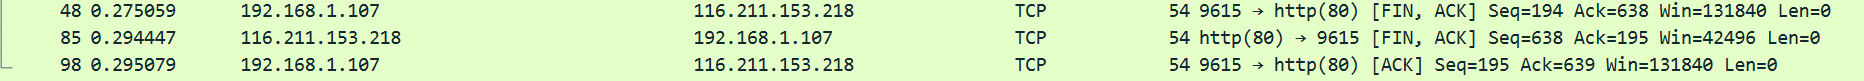
\includegraphics[width=0.95\textwidth]{img/8.png}
  \caption{四次挥手}
\end{figure}

四次挥手协议的时序图如下:

\begin{figure}[H]
  \centering
  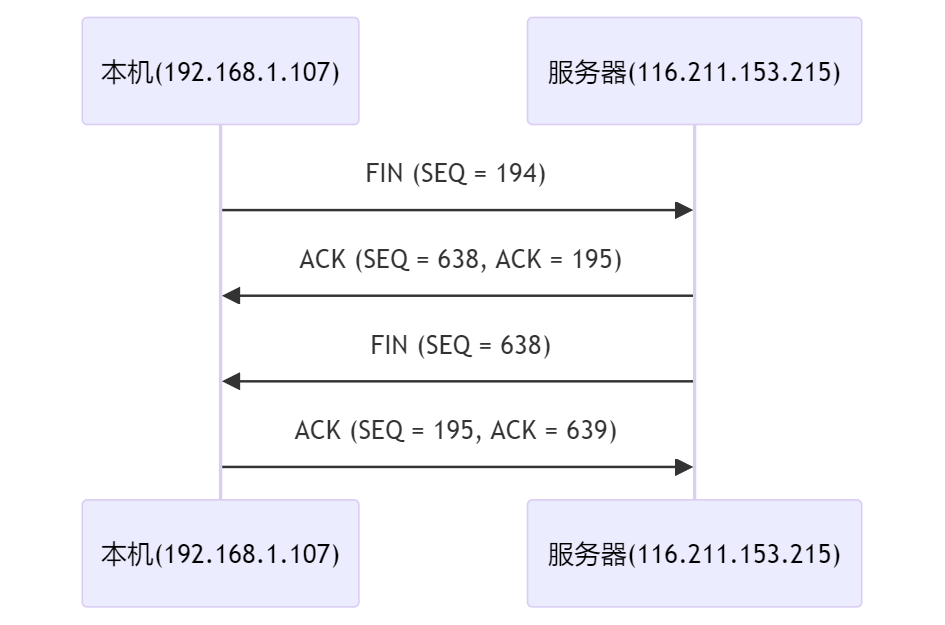
\includegraphics[width=0.95\textwidth]{img/9.png}
  \caption{四次挥手协议的步骤图}
\end{figure}

\subsection{TCP 数据传输}

通过你对数据传输的理解,回答以下问题:

\begin{enumerate}
	\item 实验中下载的大概速率为多少?(以\texttt{packets/s}和\texttt{bits/s}为单位)
	
	答:观察 \texttt{Wireshark} 生成的 \texttt{IO} (下载)图表, 如下所示:
	
	\begin{figure}[H]
		\centering
		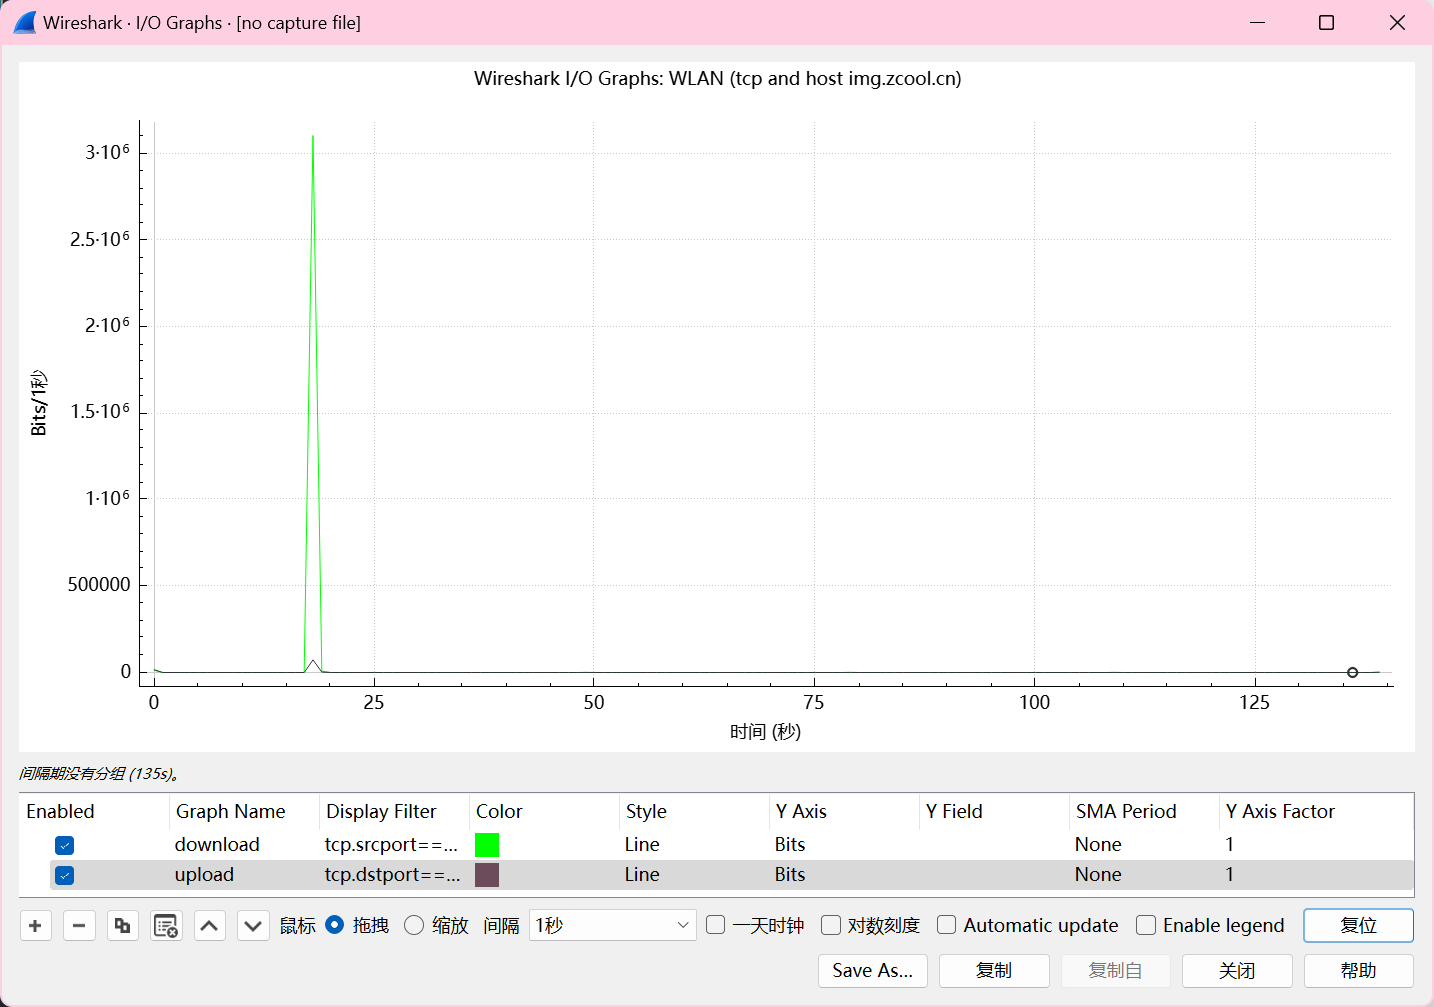
\includegraphics[width=0.9\textwidth]{img/10.png}
		\caption{\texttt{IO} (下载)图表}
	\end{figure}
	
	所以,下载速度为 \texttt{3107000 \texttt{bits/s}}。
	
	\item 下载内容(即\texttt{TCP}有效负载)占下载率的百分比是多少?
	
	答:使用\texttt{tcp.srcport==80} 进行过滤,在中间位置选择一个较大的包,分析数据如下:总的数据量为1374B,TCP携带的内容为1320B,所以内容占下载率的96.10%。
	
	\item 实验中上传的大概速率为多少?(以\texttt{packets/s}和\texttt{bits/s}为单位)
	
	答:观察 \texttt{Wireshark} 生成的 \texttt{IO} (上传)图表, 如下所示:
	
	\begin{figure}[H]
		\centering
		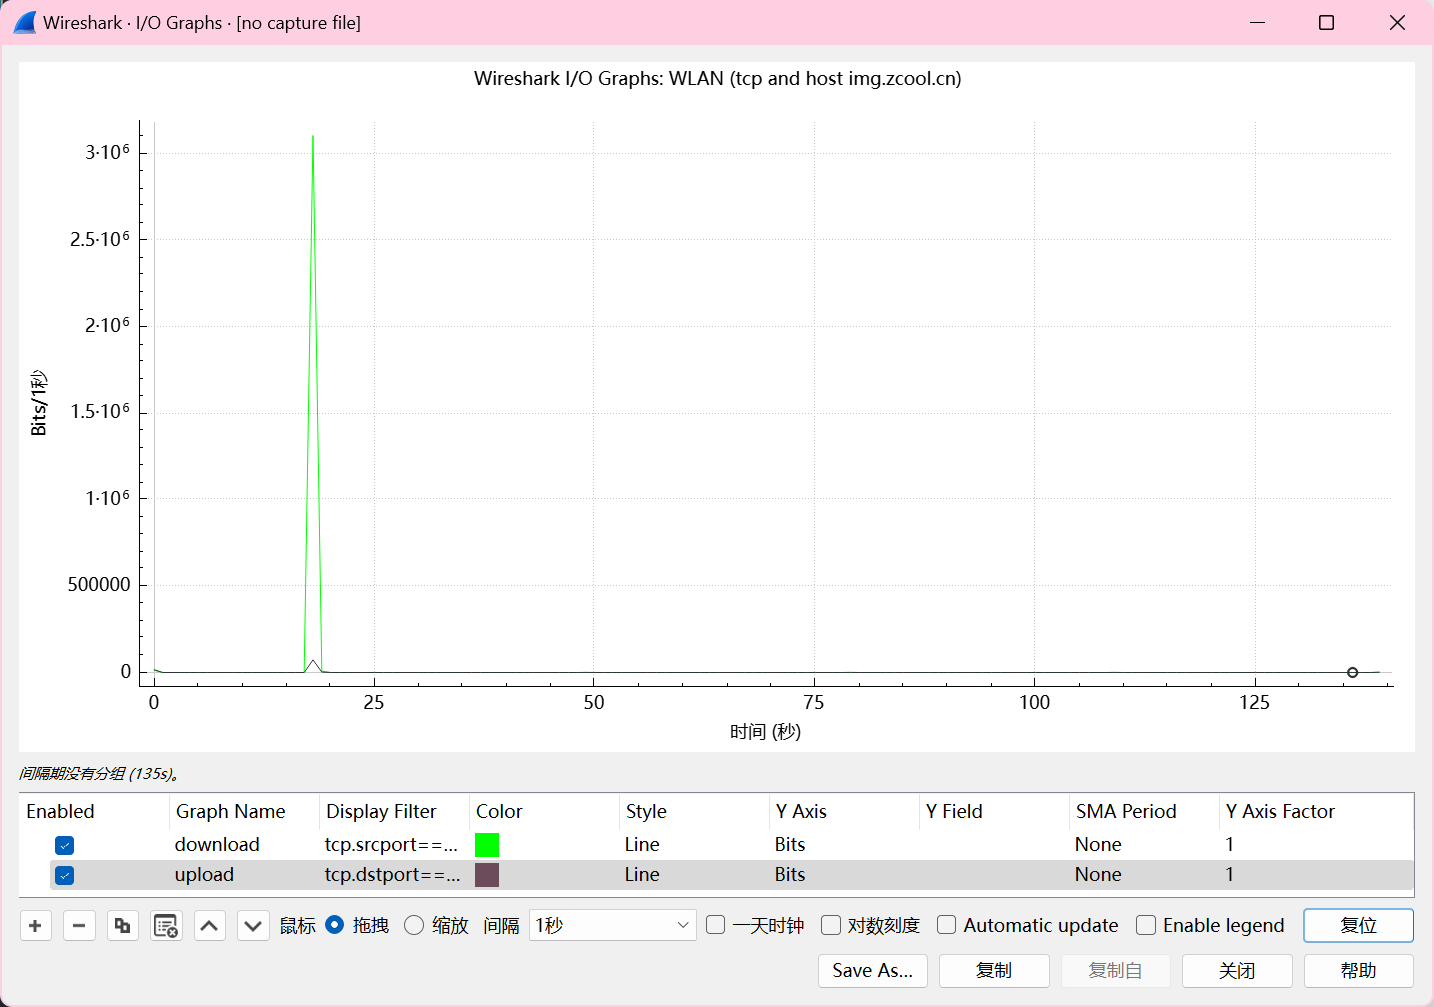
\includegraphics[width=0.9\textwidth]{img/10.png}
		\caption{\texttt{IO} (上传)图表}
	\end{figure}
	
	所以,上传速度为 \texttt{732900 \texttt{bits/s}}。
	
	\item 如果最近从服务器收到的 \texttt{TCP} 数据段的序列号是 $X$,那么下一个发送的 \texttt{ACK} 是多少?
	
	答:下一个发送的 \texttt{ACK} 是 $X + \texttt{Segment Len}$
\end{enumerate}

\subsection{继续探索\texttt{TCP}协议}

下载一个大文件,观察 \texttt{TCP} 流图表,如下所示:

\begin{figure}[H]
  \centering
  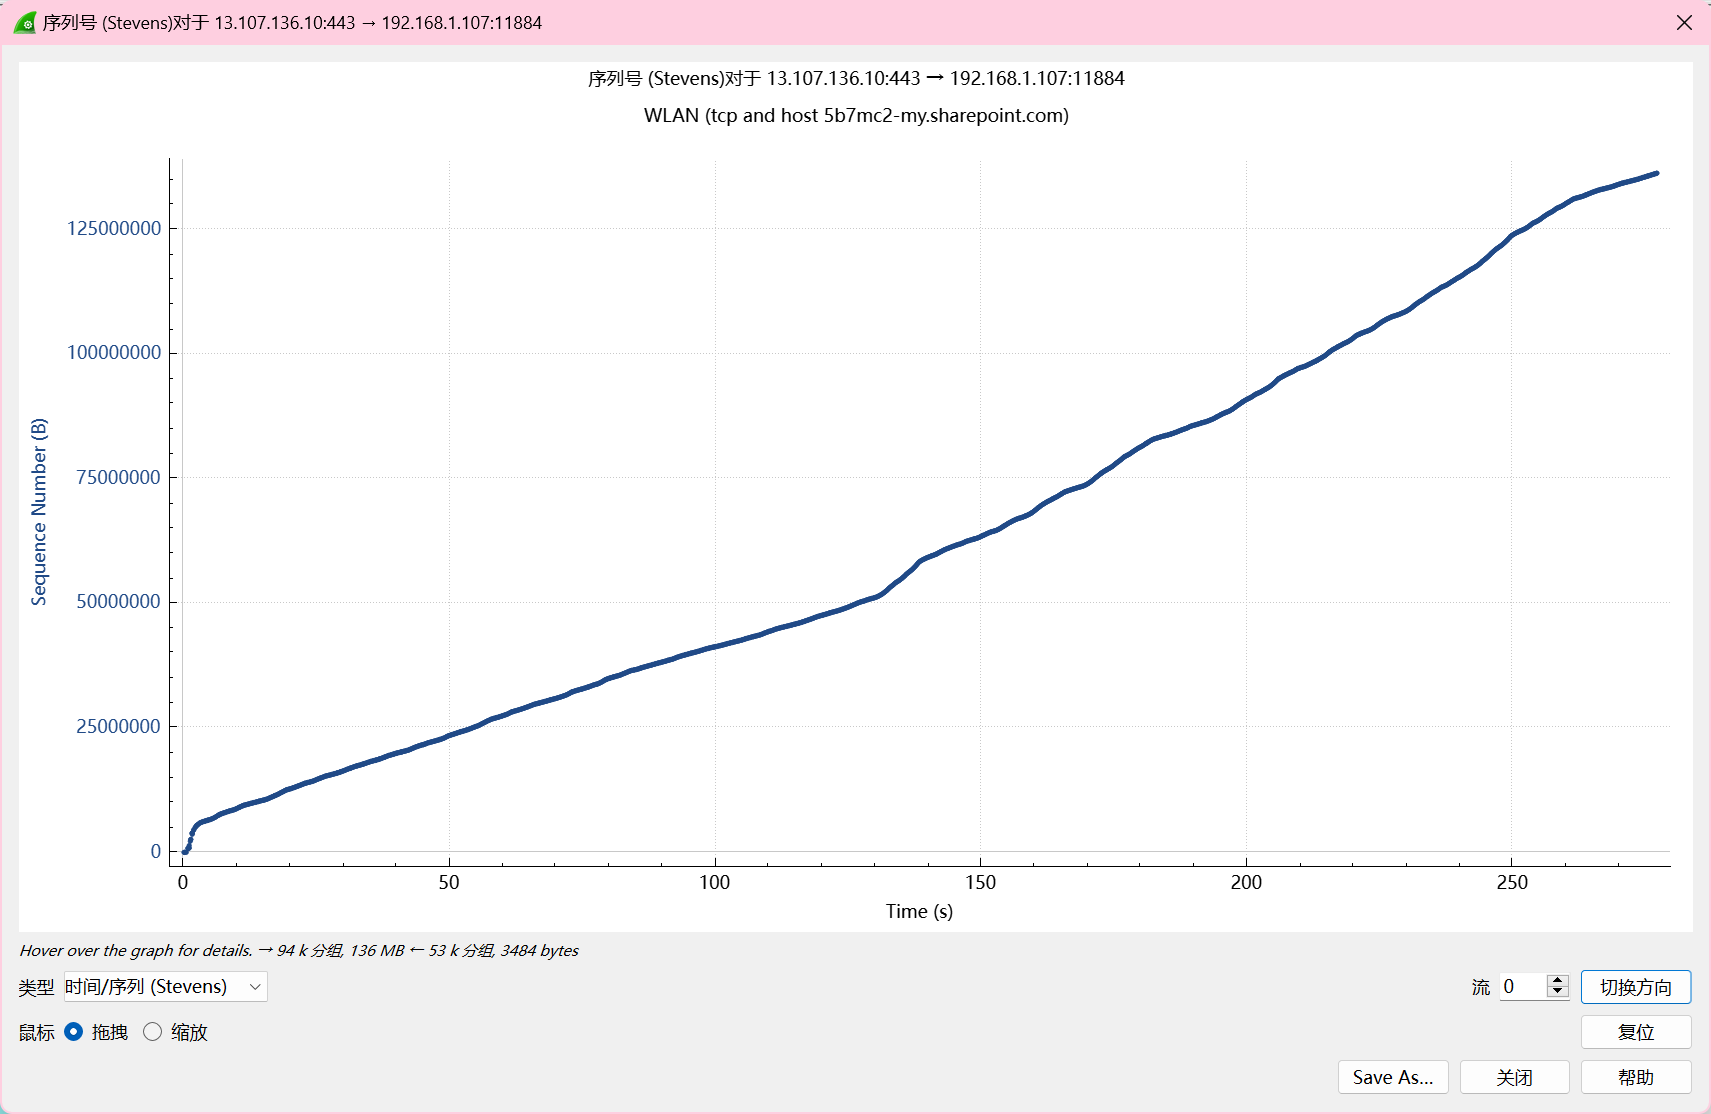
\includegraphics[width=0.8\textwidth]{img/11.png}
  \caption{序列号}
\end{figure}

\begin{figure}[H]
  \centering
  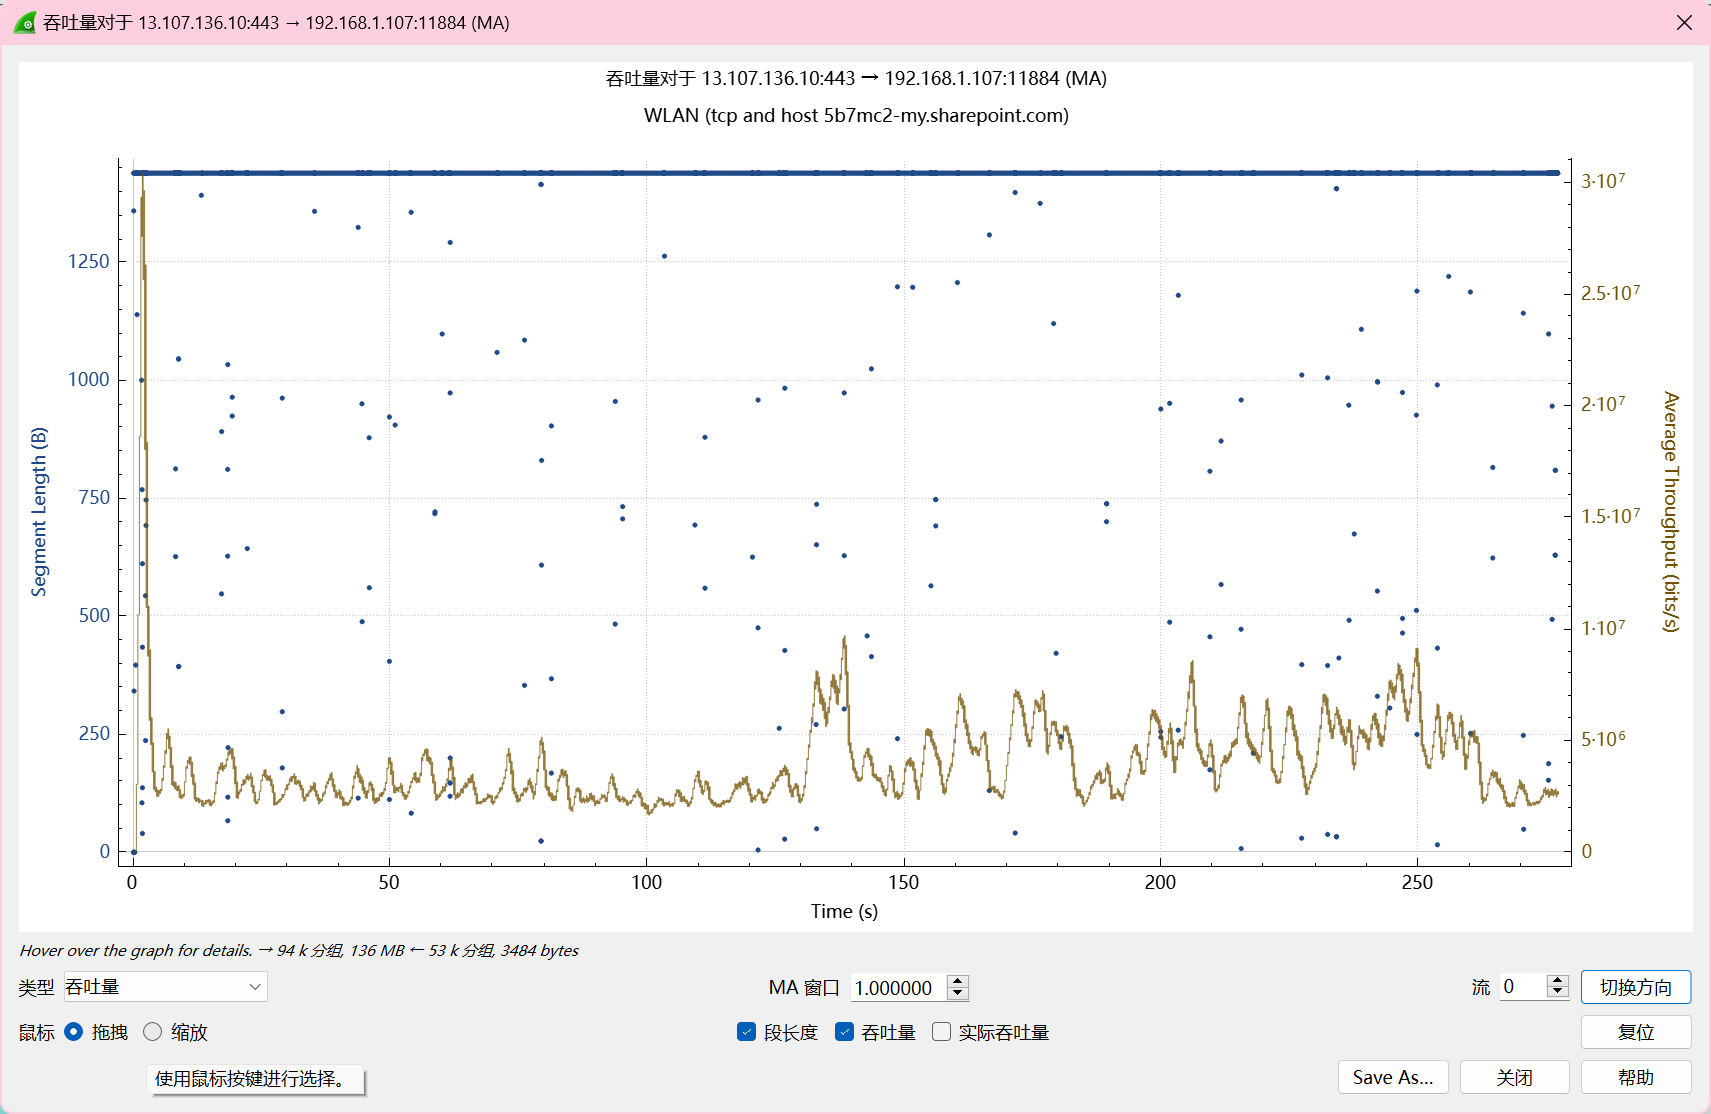
\includegraphics[width=0.8\textwidth]{img/12.png}
  \caption{吞吐量}
\end{figure}

\begin{figure}[H]
  \centering
  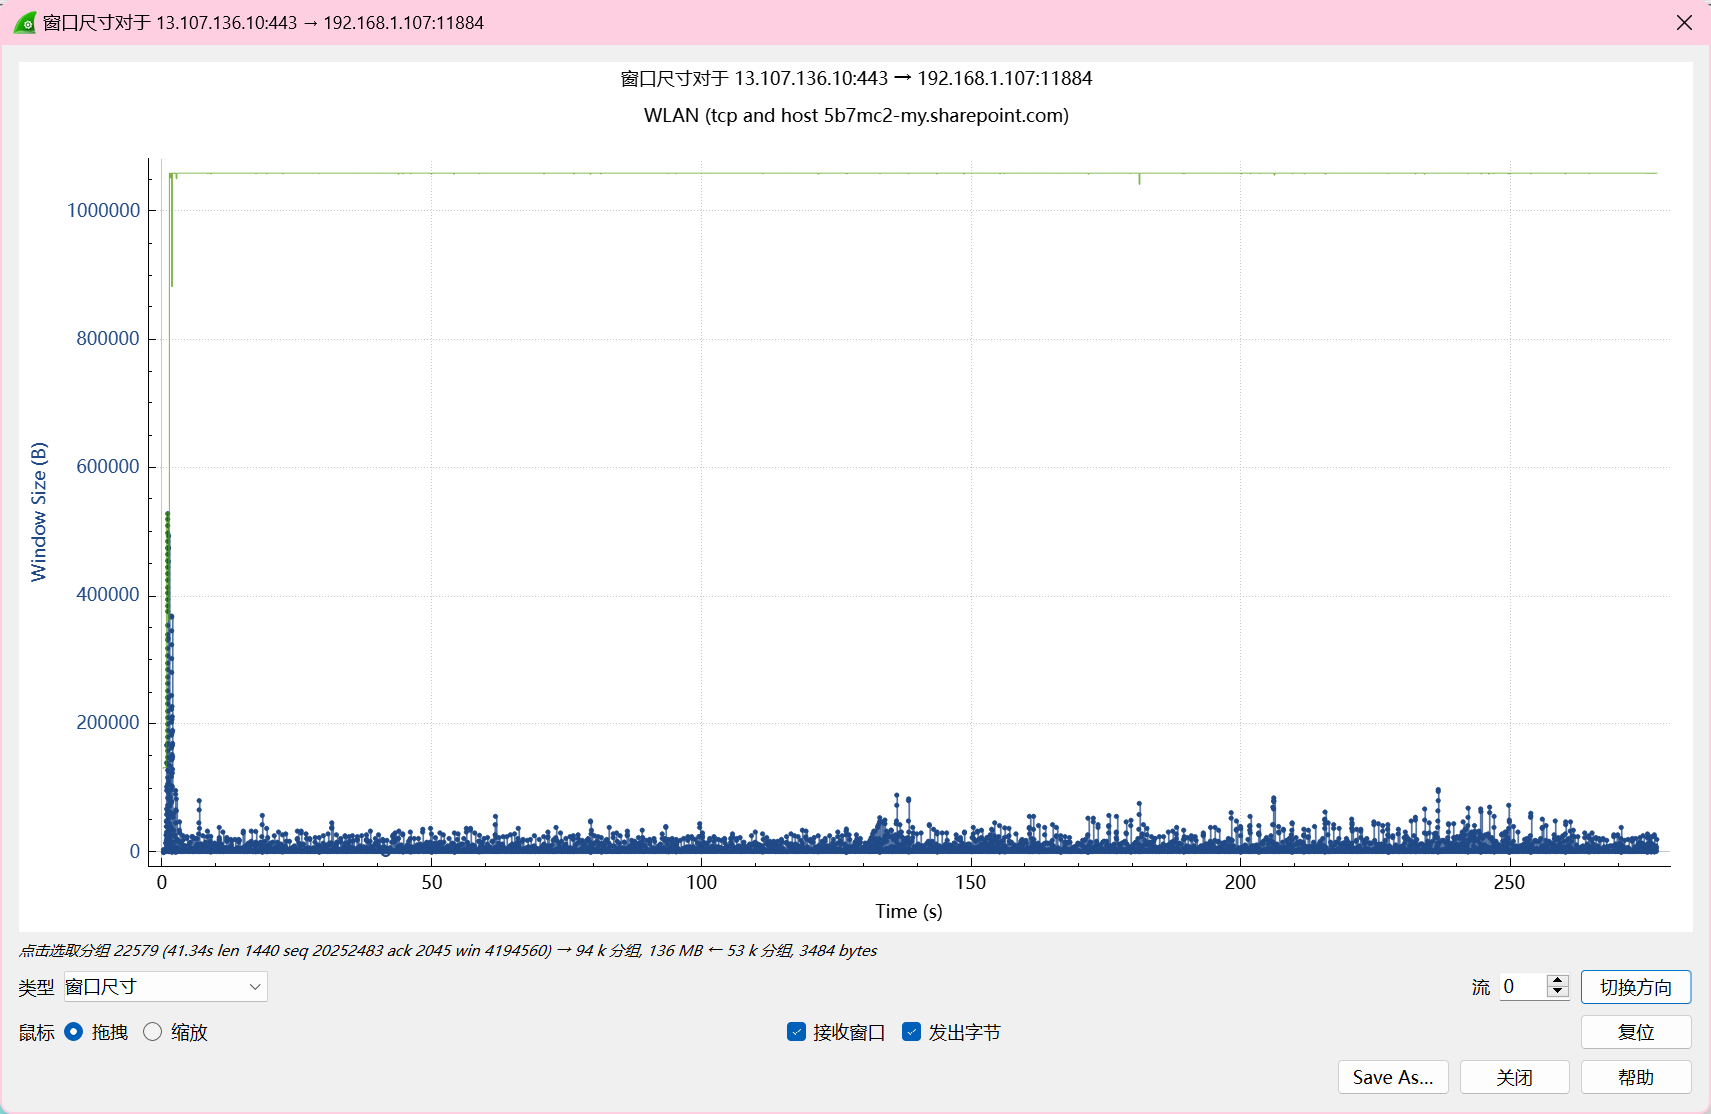
\includegraphics[width=0.8\textwidth]{img/13.png}
  \caption{窗口尺寸}
\end{figure}

\begin{figure}[H]
  \centering
  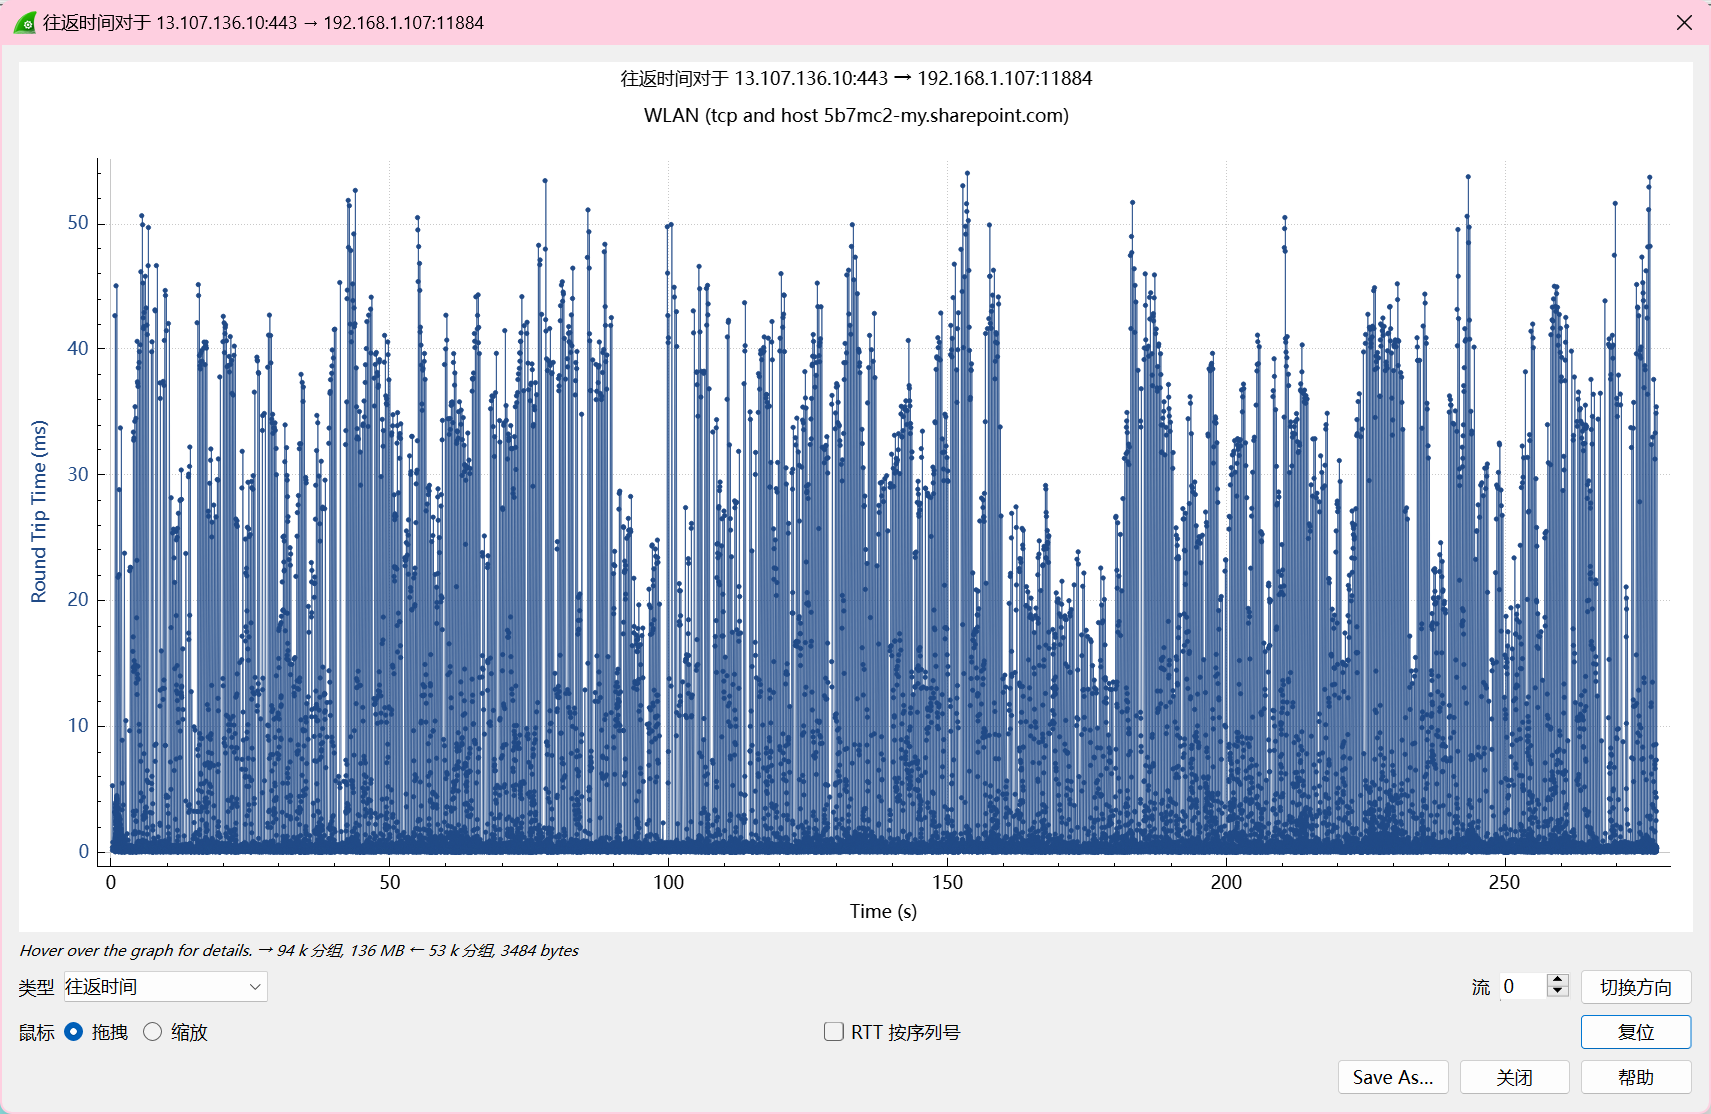
\includegraphics[width=0.8\textwidth]{img/14.png}
  \caption{往返时间}
\end{figure}

回答下列问题:

\begin{enumerate}
  \item 探索\texttt{TCP}的拥塞控制和经典\texttt{AIMD}策略。
        
  答:从吞吐量图表中可以看出,吞吐量随着时间的增加而增加,但是在某些时刻会突然下降,不断波动,这是因为在这些时刻发生了拥塞,\texttt{TCP} 会减小拥塞窗口,然后再慢慢增加,这就是拥塞控制的过程。
  
  \item 更深入地探索\texttt{TCP}的可靠性机制。捕获包括段丢失的\texttt{TCP}连接,查看什么触发重新传输以及何时触发,另外查看往返时间估算工具。

  答:可以看到,当接受到的数据包顺序错误时(可能是之前的数据包丢失了),会触发重传机制,重传丢失的数据包。

  \begin{figure}[H]
    \centering
    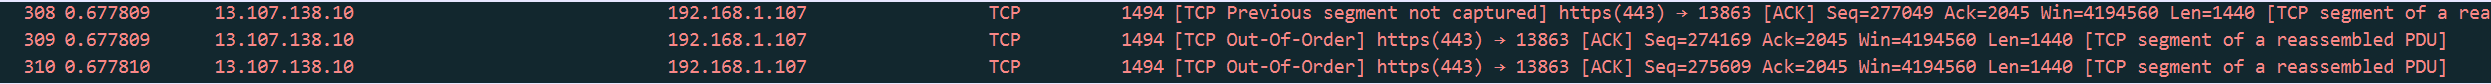
\includegraphics[width=0.95\textwidth]{img/15.png}
    \caption{错误重传}
  \end{figure}

  往返时间图表已在上方列出。
  
  \item 查看包括\texttt{SACK}在内的选项的使用以了解详细信息。

  观察一个 \texttt{Options} 中包含了 \texttt{SACK} 的数据包,如下图所示:

  \begin{figure}[H]
    \centering
    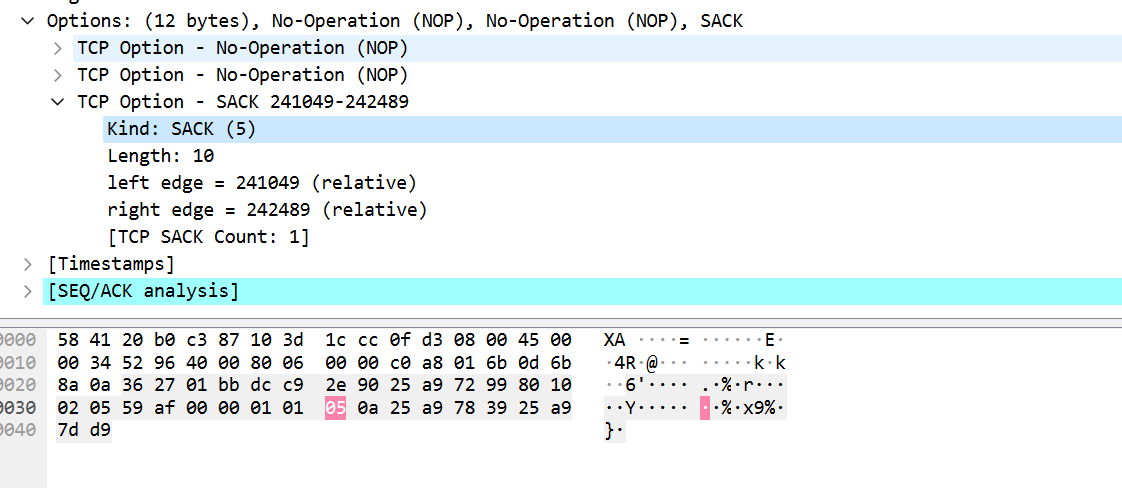
\includegraphics[width=0.8\textwidth]{img/16.png}
    \caption{\texttt{SACK}}
  \end{figure}

  可以看到,\texttt{SACK} 中包含了丢失的数据包的序列号范围。
  
  \item \texttt{TCP}是\texttt{Web}的基础传输层。可以通过设置并发连接来查看浏览器如何使用\texttt{TCP}。

  答:浏览器处理用户请求时,会建立多个 \texttt{TCP} 连接,并发地处理用户请求。

\end{enumerate}

\section{实验结果总结}

本次计算机网络实验围绕 \texttt{TCP} 展开,让我对其有了深入且全面的理解。

在实验过程中,我运用 \texttt{Wireshark} 和 \texttt{wget} 工具,成功捕获并分析了 \texttt{TCP} 报文,清晰绘制出 \texttt{TCP} 报文段结构,明确各字段含义,这使我对 \texttt{TCP} 数据包的构成有了透彻认知。通过观察 \texttt{TCP} 连接建立的三次握手和释放的四次挥手过程,我不仅绘制出详细时序图,还深入了解到每个步骤中数据包的变化及作用,尤其是 \texttt{SYN} 数据包携带的多种重要选项,如 \texttt{MSS}、\texttt{Window Scale Option} 等,它们在优化连接性能方面起着关键作用。

在数据传输阶段,我学会从 \texttt{Wireshark} 的 IO 图表分析下载和上传速率,了解到 \texttt{TCP} 有效负载在下载率中的占比情况,还掌握了根据服务器接收的序列号确定下一个 \texttt{ACK} 值的方法。此外,通过进一步探索 \texttt{TCP} 协议,我对其拥塞控制的 \texttt{AIMD} 策略、可靠性机制(如段丢失触发重传)以及 \texttt{SACK} 选项的使用有了直观认识,并且明白了浏览器在处理 Web 请求时如何利用 \texttt{TCP} 建立并发连接。

此次实验让我深刻认识到 \texttt{TCP} 在网络通信中的核心地位和重要性,它确保了数据的可靠传输与高效交互。

\section{附录}

无

\end{document}